
\begin{figure}[ht]
    \centering
    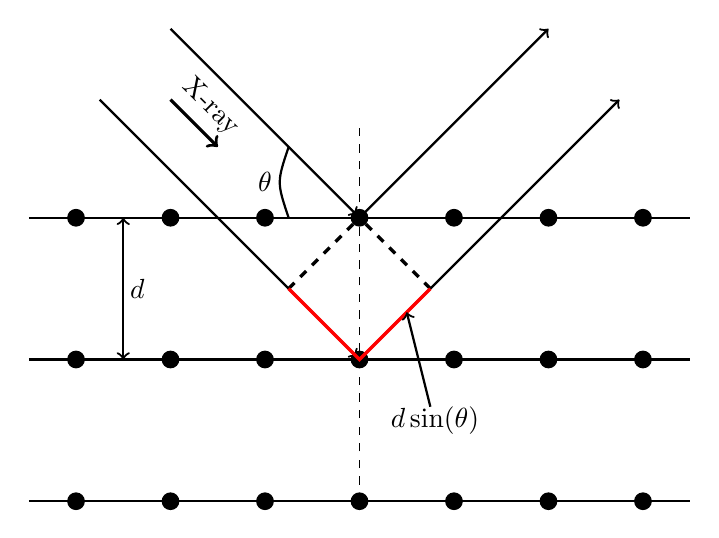
\begin{tikzpicture}[scale=0.6]
        \draw[thick] (-7,-3) -- (7,-3);
        \draw[thick] (-7,0) -- (7,0);
        \draw[thick] (-7,3) -- (7,3);
        
        %\draw (-15,-15) grid (15,15);
        \foreach \y in {-3,0,3}
            \foreach \a in {-6, -4, -2, 0, 2, 4, 6}
                \filldraw [black] (\a,\y) circle (5pt); 
        
        \draw[thick, ->] (-4, 7) -- (-0.05,3.05);
        \draw[thick, ->] (0,3) -- (4, 7);
        \draw[thick, ->] (-5.5, 5.5) -- (-0.05,0.05);
        \draw[thick, ->] (0,0) -- (5.5, 5.5); 
        
        \draw[very thick, dashed] (-1.5,1.5) -- (0,3);
        \draw[very thick, dashed] (1.5,1.5) -- (0,3);
        
        %Angle
        \draw[thick] (-1.5,4.5) .. controls (-1.75, 3.75) .. (-1.5, 3);
        \node at (-2, 3.75) {$\theta$};
        %\node at (0,3.5) {0,3};
        \draw[dashed] (0,-3) -- (0,5);
        \draw[thick,->] (-5,3) -- (-5,0);
        \draw[thick,->] (-5,0) -- (-5,3);
        \node at (-4.7, 1.5) {$d$};
        
        \draw[very thick, red] (-1.5,1.5) -- (0,0) -- (1.5,1.5); 
        \draw[thick, ->] (1.5,-1) -- (1,1);
        \node at (1.6,-1.3) {$d\sin(\theta)$};
        
        \draw[very thick, ->] (-4,5.5) -- (-3,4.5) node[midway, left, above, rotate=-45]{X-ray};
    \end{tikzpicture}
    \caption{Caption}
    \label{fig:test}
\end{figure}


\subsubsection{Electrical conduction}

It is common practice to divide materials into categories regarding their electrical properties such as insulators, semiconductors and conductors. The differences in these properties originate from the band structures described by quantum mechanics **FIGURE**

*An insulator has a completely filled valence band and an empty conduction band with a large band gap, while conductors have a  partially filled valence band (metal) or overlapped bands (semi-metal), thus helping electrons in the crystal move more easily when an external field is applied.*

%side by side
\begin{figure}
	\centering
	%\setbox1=\hbox{\includegraphics[height=8cm]{uploads/MO_lav_012-02-x250-C}}
	\includegraphics[height=6.5cm]{uploads/MO_lav_012-02-x250-C}\llap{\raisebox{4cm}{\includegraphics[height=2.5cm]{uploads/MO_lav_mulig_inset_012-02-x1800-C}}}
	\includegraphics[height=6.5cm]{uploads/MO_hoy_023-02-x250}\llap{\raisebox{4cm}{\includegraphics[height=2.5cm]{uploads/MO_hoy_mulig_inset_023-02-x1800}}} 
	\caption{SEM images of synthesized \ce{MnO2} with (i) a 0.252 M concentration of cations and (ii) a 2.5 M concentration of cations. Something about coverage}
	\label{fig:my_label}
\end{figure}


%side by side with letter on side and inlet
\begin{figure}
    \begin{subfigure}[t]{0.02\textwidth} \raisebox{6cm}{a)} \end{subfigure}
	\begin{subfigure}[b]{0.48\textwidth}
	\includegraphics[height=6.5cm]{uploads/MO_lav_012-02-x250-C}\llap{\raisebox{3.5cm}{\includegraphics[height=3cm]{uploads/MO_lav_mulig_inset_012-02-x1800-C}}}
	\end{subfigure}
    \begin{subfigure}[t]{0.02\textwidth}
    \raisebox{6cm}{b)}
    \end{subfigure}
	\begin{subfigure}[b]{0.48\textwidth}
	\includegraphics[height=6.5cm]{uploads/MO_hoy_023-02-x250}\llap{\raisebox{3.5cm}{\includegraphics[height=3cm]{uploads/MO_hoy_mulig_inset_023-02-x1800}}} 
	\end{subfigure}
	\caption{SEM images of the synthesized \ce{MnO2} with (a) a 0.252 M concentration of cations and (b) a 2.5 M concentration of cations. Something about coverage. And mention the inlet?}
	\label{fig:MnO2_diff}
\end{figure}


\begin{figure}
    \begin{subfigure}[t]{0.02\textwidth} \raisebox{6cm}{a)} \end{subfigure}
	\begin{subfigure}[b]{0.98\textwidth}
	\includegraphics[height=6.5cm]{uploads/MO_lav_012-02-x250-C} \includegraphics[height=6.5cm]{uploads/MO_lav_mulig_inset_012-02-x1800-C}
	\end{subfigure} \\ [-1em]
    \begin{subfigure}[t]{0.02\textwidth}
    \raisebox{6cm}{b)}
    \end{subfigure}
	\begin{subfigure}[b]{0.98\textwidth}
	\includegraphics[height=6.5cm]{uploads/MO_hoy_023-02-x250} \includegraphics[height=6.5cm]{uploads/MO_hoy_mulig_inset_023-02-x1800}
	\end{subfigure}
	\caption{SEM images of the synthesized \ce{MnO2} with a a) 0.252 M concentration of cations and b) 2.5 M concentration of cations  As can be seen by comparing a) and b), the coverage has increased significantly with the increased concentration of precursors. And mention the inlet?}
	\label{fig:MnO2_diff}
\end{figure}


\begin{table}[ht]
    \centering
    \caption{Table of different parameters and their effect on the synthesis.}
    \resizebox{\textwidth}{!}{
    \begin{tabular}{c c c}
    \hline
        Parameter & implemented change & observed effect \\
        Position of needle & Moved needle 1 cm up and 2 cm down from starting point & No visible effect \\
        Concentration of precursors & The 1st concentration was doubled then further increased by a factor of 10 & Both particle size and amount of deposited material increased \\
    \hline
    \end{tabular} }
    \label{tab:parameters}
\end{table}